\documentclass[final]{siamltexmm}
\documentclass[10pt,a4paper]{article}

\usepackage{graphicx}
\usepackage{algorithm}
\usepackage{algorithmic}

% \usepackage[demo]{graphicx}
% \usepackage{subfig}

\newcommand{\pe}{\psi}
\def\d{\delta} 
\def\ds{\displaystyle} 
\def\e{{\epsilon}} 
\def\eb{\bar{\eta}}  
\def\enorm#1{\|#1\|_2} 
\def\Fp{F^\prime}  
\def\fishpack{{FISHPACK}} 
\def\fortran{{FORTRAN}} 
\def\gmres{{GMRES}} 
\def\gmresm{{\rm GMRES($m$)}} 
\def\Kc{{\cal K}} 
\def\norm#1{\|#1\|} 
\def\wb{{\bar w}} 
\def\zb{{\bar z}} 

% some definitions of bold math italics to make typing easier.
% They are used in the corollary.

\def\bfE{\mbox{\boldmath$E$}}
\def\bfG{\mbox{\boldmath$G$}}

\title{Independent Study -- Song Structure with Spectral Clustering}
\author{Peter Yun-shao Sung\thanks{\tt yss265@nyu.edu} }

\begin{document}
\maketitle

\begin{Note}
This is independent study mid-way report
\end{Note}

\pagestyle{myheadings}
\thispagestyle{plain}

\section{Abstract}
There are many approaches to understand the structure of music, and this is a project applying spectral graph theory with Laplacian formula to analyze repeated patterns in musical recordings. Starting with low-dimensional encoding of repeating structure, hierarchical relationship among repeating components will be built by changing number of eigenvectors. Further works for this project will include Neural Network and back-propagation to apply thie technique to analyze the structure of wide variety of musics.

\\
\section{Baseline Approach}
Here is the baseline approach which can be roughtly divided into two parts: the goal of the first part is constructing \textit{sequence-augmented affinity matrix A} from \textit{symmetric matrix R} of the feature similarity at each time points, and the second part is to construct symmetric normalized Laplacian matrix and obtain the top $m$ eigenvectors with the $m$ smallest eigenvalues, and then perform k-means for boundary detection. The high level pseudocode is described in Algorithm 1.

\begin{algorithm}[htb]
  \caption{Baseline Approach}
  \SetKwInOut{Input: }{number of top $m$ smallest eigenvalues}
  \label{algo:SC}
\begin{algorithmic}[1]
  \STATE M = getSymmetricMatrix() //to get affinity matrix
  \STATE L = scipy.sparse.csgraph.laplacian(M) //to get symmetric normalized Laplacian matrix
  \STATE eigVals, eigVecs = np.linalg.eig(L)
  \STATE Y = getMthSmallest(eigVals, eigVecs, m)
  \STATE return boundaryDetection(Y)
\end{algorithmic}
\end{algorithm}


\subsection{Symmetric and Laplacian Matrix}
Initially symmetric matrix is constructed manually, and the symmetric properity is ensured by checking $m == m^T$. The following symmetric normalized Laplacian L is defined as:
\begin{equation}
L = I - D^{-1/2}AD^{-1/2}
\end{equation}
The properity of symmetric is important as it shows the correlation between time $i$ and $j$ which is an undirected graph, and the proterity is important to hold to make sure the eigenvectors calculated from Laplacian matrix is done correctly. Figure 2.1 shows the example of symmetrix matrix and its corresponding top-10 eignevectors, and method is implemented from Algoritm 1.

\begin{figure}[H]
\centering
\begin{subfigure}
  \begin{tabular}{c}
  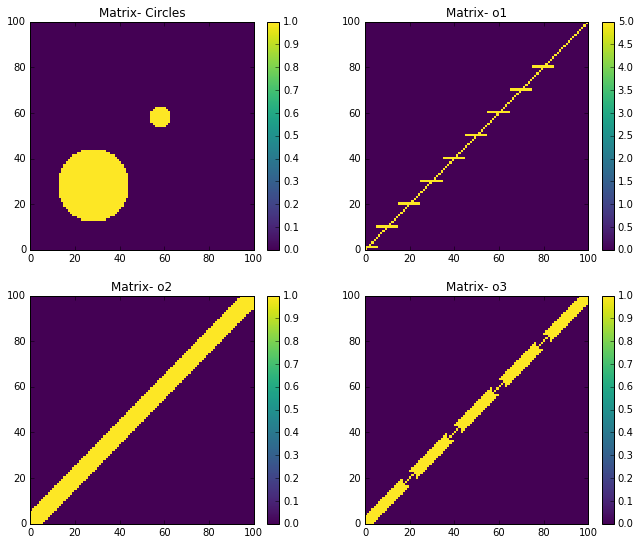
\includegraphics[width=50mm]{./figure/similarityMatrix.png}
  \end{tabular}{}
\end{subfigure}
  \begin{tabular}{c}
  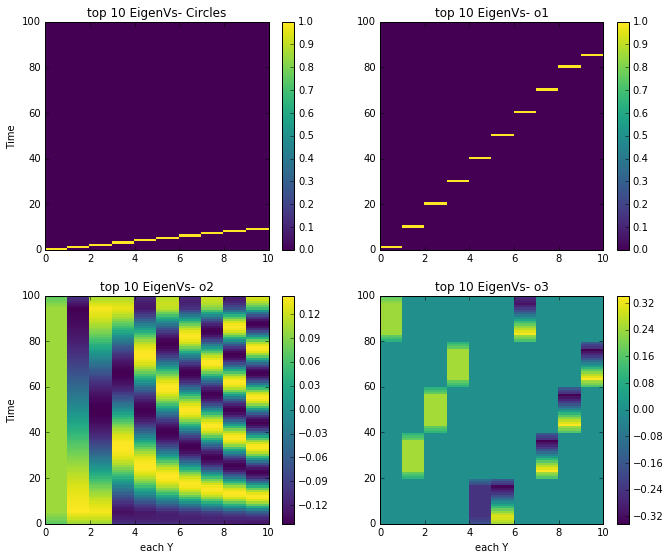
\includegraphics[width=50mm]{./figure/similarityMatrix_eigens.png}
  \end{tabular}{}
\begin{subfigure}
\end{subfigure}
\caption{Symmetric matrixs and corresponding eigen vectors. Left: four different type of symmetirc matrix, and Right: the top-10 eigen vectors}
\end{figure}
Interestingly, eigenvectors are like the building blocks of the original graph, and the signal of each eigenvector are like showing the correlation of each time point in this building block. As the top-m eigenvectors matrix $Y$ constructed, we can notice from Figure 2.2 that the dot product of $YY^T$ is similar to the original symmetric matrix, although in low-resolution way but a good fit to the purpose of finding the structure. I think understand the properity of eigenvector is important, as the each row from $Y$ is similar to the eigen-feature representation at each time point, and therefore we can perform k-means for boundary detection based on $Y$ as illustrated in Algorithm 2.
\begin{figure}[H]
  \centering
    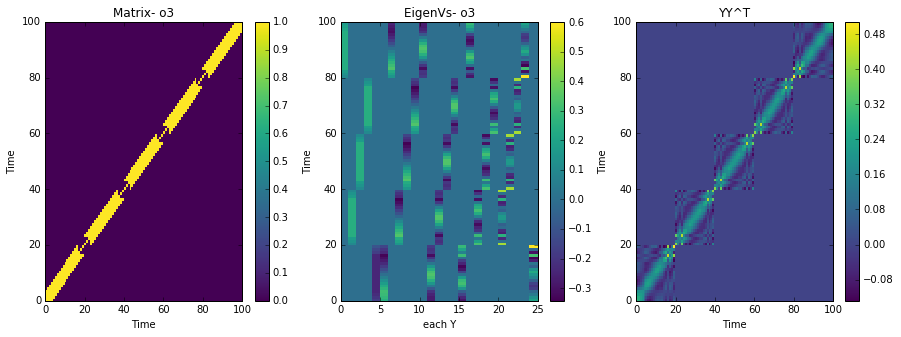
\includegraphics[width=0.8\textwidth]{./figure/o3_eachStage.png}
  \caption{The steps from symmetric matrix to eigenvector: R, Y, $YY^T$}
\end{figure}


\subsection{Boundary Detection}
As the pseudocode shown in Algorithm 2, once the Laplacian matrix is constructed, each row is the representation of eigen-features at specific time. Therefore, running k-means for eigen-features of all time points will yield the results of which centroids of this time point belongs to, and therefore the place where the $t_{i} \neq t_{i+1}$ is where the boundary is. As showed in Figure 2.3, boundary is correctly detected at each time point, but when doing experiments I noticed the number of iteration during k-means will affect the correctness of boundary, and the more iteration usually gives better boundary.
\begin{figure}[H]
\centering
\begin{subfigure}
  \begin{tabular}{c}
  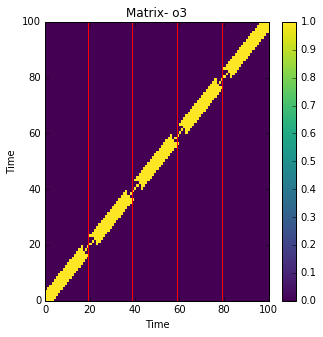
\includegraphics[width=25mm]{./figure/o3_boundary.png}
  \end{tabular}{}
\end{subfigure}
  \begin{tabular}{c}
  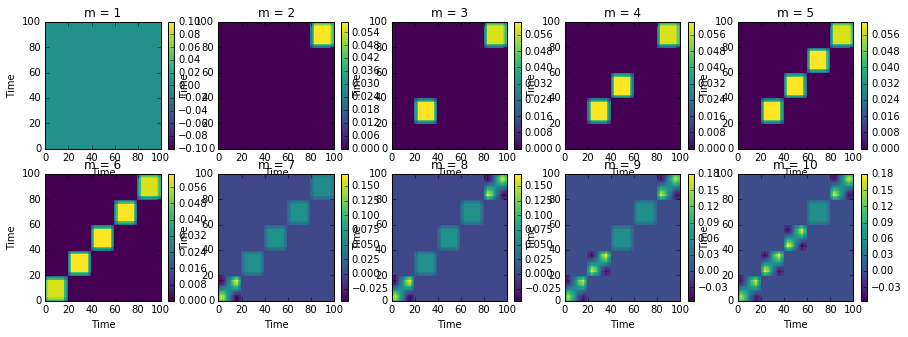
\includegraphics[width=75mm]{./figure/o3_eachM.png}
  \end{tabular}{}
\begin{subfigure}
\end{subfigure}
\caption{Boundary detection and pair-wise frame similarities ($YY^T$). Left: Boundary detection of original recurrence graph, and Right: visualization of $YY^T$ using the first 10 eigenvectors}
\end{figure}

\begin{algorithm}[htb]
  \caption{boundaryDetection}
  \SetKwInOut{Input: }{Laplacian eigenvectors $Y \in \mathbb{R^{n \times m}}$}

  \SetKwInOut{Output: }{Boundary b, Centroids c}
  \label{algo:SC}
\begin{algorithmic}[1]
  \STATE $ \overline y_i = \frac{Y_i}{\parallel Y \parallel}$ //normalize each row $Y_i$
  \STATE Run k-means on $\{ \overline y_i \}_{i=1}^{n}$
  \STATE Let $c_i$ denote the cluster containing $ \overline y_i$
  \STATE $b \leftarrow \{ i|c_i \neq c_{i+1}\}$
  \STATE return b, c
\end{algorithmic}
\end{algorithm}

\subsection{Affinity Matrix from Real Music}
As basic process is established above, I started to construct matrix from real music, and the music I started with is \textit{The Beatles - Come Together}. Data is sampled in the rate of 22050Hz, and transformed to .wav format, as it can be imported by scipy. Imported signal has two tracks, and all following analysis is based on the first track, and feature extraction is done by librosa cqt computing the constant-Q transform of an audio signal. As we will get too little information at low frequencies and too much information at high frequencies if we just simply double the frequency for Fourier transformation[Ref 6], and cqt will be better suit for extracting feature from music signal because it spaced the center frequencies of the frequency bins geometrically, and Q-factors are all equal[Ref 7]. As we can see from Figure 2.4, feature extraction from mfcc and cqt is different and seems cqt is able to cpature long-range repeating form.

\begin{figure}[H]
\centering
\begin{subfigure}
  \begin{tabular}{c}
  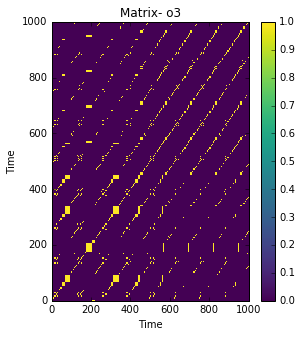
\includegraphics[width=40mm]{./figure/cqt.png}
  \end{tabular}{}
\end{subfigure}
  \begin{tabular}{c}
  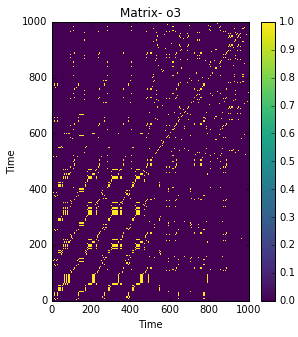
\includegraphics[width=40mm]{./figure/mfcc.png}
  \end{tabular}{}
\begin{subfigure}
\end{subfigure}
\caption{Visualization of recurrence graph $R$ from matrix in Figure 2.3 after Left: cqt and Right: mfcc feature extraction}
\end{figure}

The \textit{affinity matrix A} is constructed by:
\begin{equation}
A_{ij} = \mu R^{\prime}_{ij}S^{rep}_{ij} + (1-\mu)\Delta_{ij}S^{loc}_{ij}
\end{equation}
where $R_{ij}$ is recurrence matrix and $R[i][j]$ is 1 if time $i$ and $j$ are mutual k-nearest neighbors else is 0, and $R$ is symmetric. $\Delta[i][j]$ is 1 if $|i-j|=1$ else is 0. $S_{ij}$ is the result of matrix passed to $Gaussian Kernel$ of feature vectors $x_i$, $x_j$:
\begin{equation}
G(M) = S_{ij} = exp\left( {-1\over2\sigma^2} \|x_i-x_j\|^2  \right) \textbf{, for each row of i and j in M}
\end{equation}
and $S^{rep}_{ij} = G(R^{\prime}_{ij})$ and $S^{loc}_{ij} = G(\Delta_{ij})$, and $\mu$ in Equation 2.2 is a factor balancing local and global linkage, and optimal of $\mu$ is solved by:
\begin{equation}
\mu^{\ast} = {<d(\delta), d(R^{\prime})+d(\delta) >\over \|d(r^{\prime})+d(\delta)\|^2}
\end{equation}
where we treat the input matrix as vector of degree-sum where $d(\cdot)=[d_i(\cdot)]^n_{i=1}$, and $d_i(G) = \Sigma_jG_{ij}$ is the degree sum at time $i$. However, after the affinity matrix $A$ being constructed from Equation 2.2, we loss the symmetric proerity, even though $R^{\prime}_{ij}, S^{rep}_{ij}, \Delta_{ij}, S^{loc}_{ij}$ are symmetric. The product from matrix multiplication from Equation 2.2 is not symmetric, and the addition modification may be required. Figure 2.5 is the visulization for $R$, $A$, and $Y$ with the top 25 eigenvectors.

\begin{figure}[H]
  \centering
    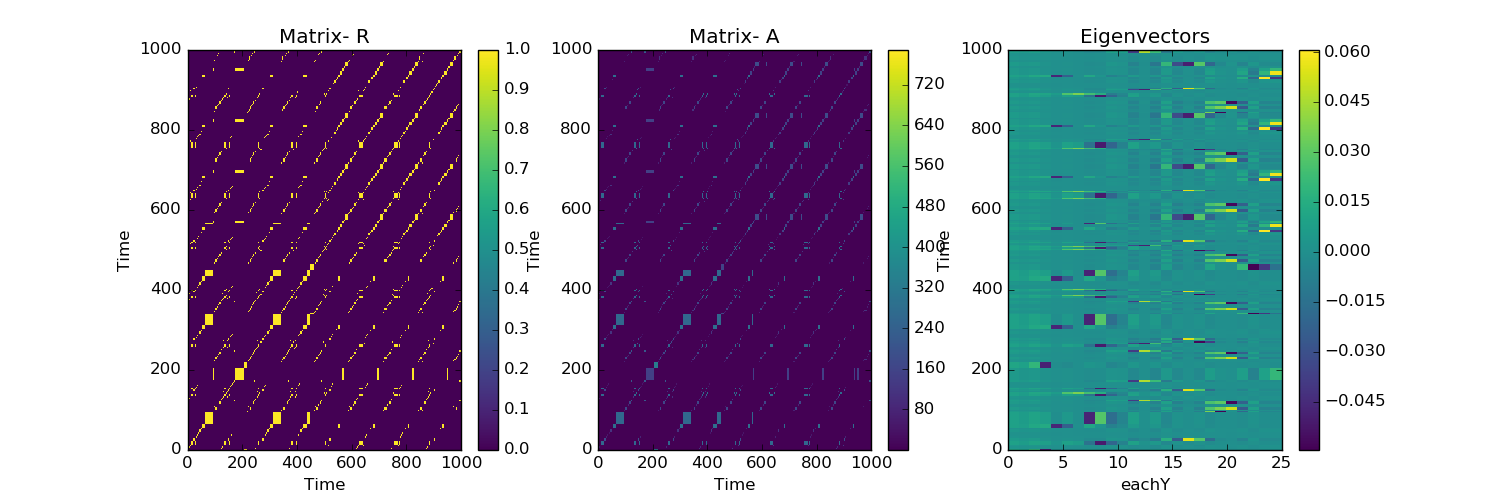
\includegraphics[width=1\textwidth]{./figure/allMatrix.png}
  \caption{First 1000 time point of recurrence and affinity matrix, and first 25 eigenvectors for The Beatles - Come Together}
\end{figure}


\section{Discussion}
Here is the section for discussion about the current issues.\\
The first issue is about the time complexity. Input signal of a 3 minutes music contains 6291012 data points and still 12288 points after mfcc or cqt, which gives us a recurrent matrix $R$ in shape of (12288, 12288). For a graph matrix like this big shape will give a hard time for visualizing the whole matrix, as well as spending lots of time on calculations like Equation 2.3 which is an $O(n^2)$. Also, np.linalg.eig, line 3 in Algorithm 1 is requiring computation time, and line 4 in Algorithm 1 also requiring sorting since the returned eigen value form line 3 doen't guarantee in sorted order. I think these complexity is one of the reason that motivate Ref 4 to use encode and decode method, but the advantage of our method is able to understange the hierarchical structure which is different from Ref 4. The majority vote method mentioned in Ref 2 maybe will be a way to reduce the shape of the matrix, but addition clarification may needed to implement this method.\\
The second issue is about the construction of affinity matrix $A$ in Equation 2.2. We loss the symmetric properity after $A$ constructed, mainly due to the fact that matrix multiplication is not guarantee the symmetric properity.

\section{Further Works}
The goal of this project is to further construct \textit{Convolutional Neural Network} (CNN) on-top of the Laplacian formula that we have constructed above. There are many different approaches using techniques like decode-encode and embeddings in Ref 8 and Ref 3 respectively. However, although the methods can successfully perform boundary detection and maybe efficient than Laplacian, I think we will loss hierarchical meaning if we are using their method.

Dr. LeCun's paper in Ref 8 described method for Multiresolution Analysis on Graphs for data with weak geometric structure, and there they also extend the analysis via Laplacian Spectrum. Although the method may related to our works, addtional evaluation may need to make sure we can apply thier method to perform boundary detection on musical recording as well as preserving its hierchical meaning.

In a web tutorial that explaining the CNN architecture for Spotify music recommendation, they performed multiple convolutional layers followed by fully connected networks. I think the convulutional layworks is worth trying since many of the filters pick up, or emphasize, harmonic content Figure 2.6, and maybe we can extract the features after several convolutional layers and form an Laplacian matrix for boundary detection. The idea to add fully connect layers is still not quite clear to me since the output from there will be only one vector which is not possible to form Laplacian matrix and perform boundary detection.
\begin{figure}[H]
  \centering
    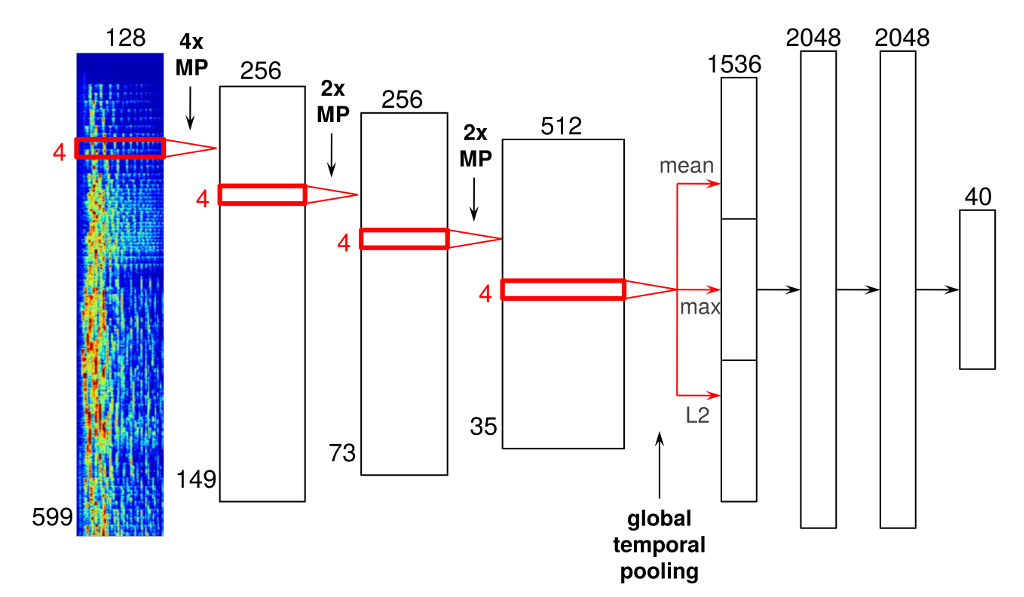
\includegraphics[width=0.5\textwidth]{./figure/spotify_convnet.png}
    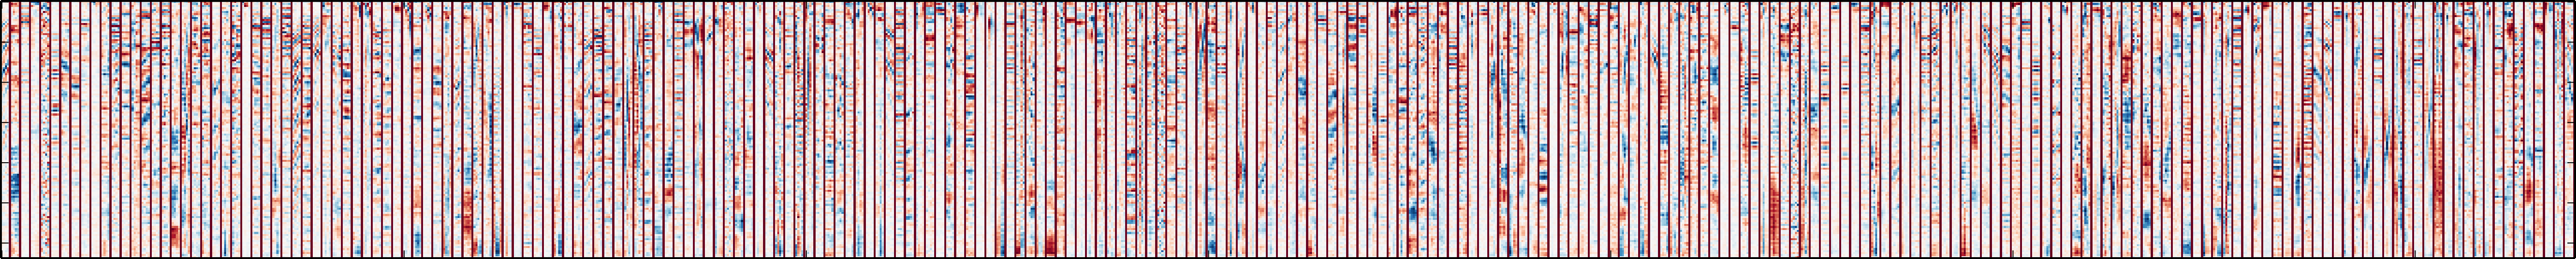
\includegraphics[width=0.7\textwidth]{./figure/filters_hires.png}
  \caption{Top: Convolutional neural network architectures at \url{http://benanne.github.io/2014/08/05/spotify-cnns.html}. Bottom: Visualization of the filters learned in the first convolutional layer}
\end{figure}


\begin{thebibliography}{10}
\bibitem{fpf} {\sc A Tutorial on Spectral Clustering}
\bibitem{fpf} {\sc Analyzing Song Structure with Spectral Clustering}
\bibitem{fpf} {\sc Deep clustering: Discriminative embeddings for
segmentation and separation}
\bibitem{fpf} {\sc Learning Deep Representations for Graph Clustering}
\bibitem{fpf} {\sc Hierarchical Evaluation of Segment Boundary Detection}
\bibitem{fpf} {\sc Calculation of a Constant Q Spectral Transformation}
\bibitem{fpf} {\sc Constant-Q Transform Toolbox for Music Processing}
\bibitem{fpf} {\sc Spectral Networks and Deep Locally Connected Networks on Graphs}
\end{thebibliography}

\end{document}
